\chapter{Konzeption\label{chap2:Zweites-Kapitel}}

Während der Konzeptionsphase ging es darum einen ersten Entwurf für die spätere Implementierung zu entwerfen. Hierfür wurden verschiedene Mockups erstellt, welche einen ersten Einblick in die Designvorstellungen für die mobile Anwendung \glqq Geogram\grqq{} geben sollen.

Mit dem Definieren der MVP-Kriterien, wurde der Funktionsumfang, für die erste minimal funktionsfähige Iteration der mobile Anwendung \glqq Geogram\grqq{} aufgelistet. Zusätzlich wurden noch weitere Soll- und Kann-Kriterien festgelegt.

\section{Mockup's\label{sec2.1:Unterpunkt-1}}

In \autoref{fig:login_white} und \autoref{fig:login_black} ist die Login-Ansicht abgebildet. Bereits als Mockup realisiert, ist der Wechsel zwischen einem White- und Dark-Mode der mobilen Anwendung.

\begin{figure}[H]
    \centering
    \begin{minipage}{.5\textwidth}
      \centering
      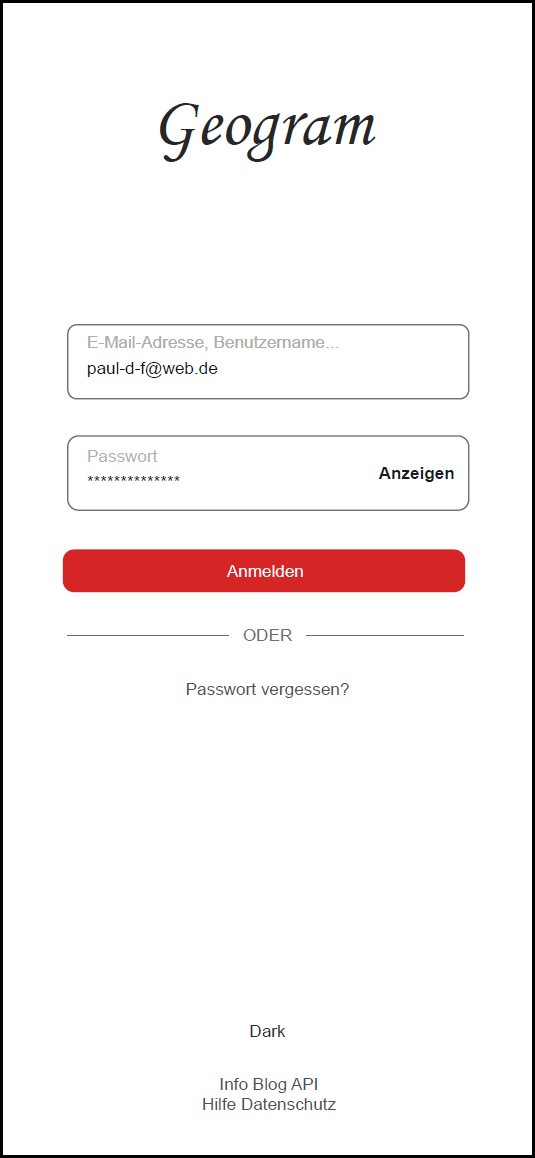
\includegraphics[width=.6\linewidth]{images/Login_MockUp.png}
      \caption{Login-Ansicht in weiß}
      \label{fig:login_white}
    \end{minipage}%
    \begin{minipage}{.5\textwidth}
      \centering
      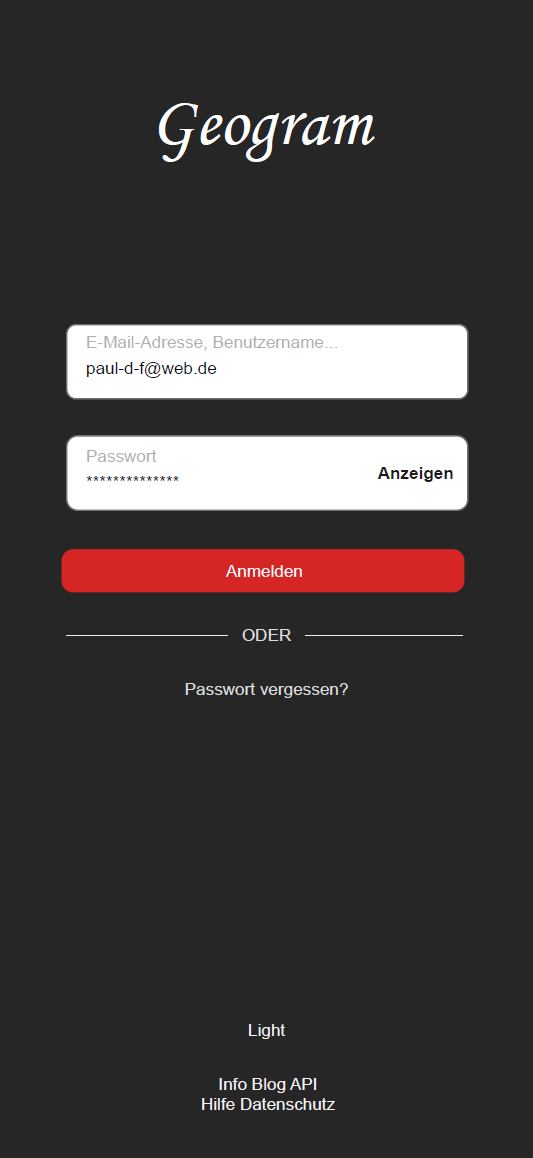
\includegraphics[width=.6\linewidth]{images/Login_MockUp_Black.png}
      \caption{Login-Ansicht in schwarz}
      \label{fig:login_black}
    \end{minipage}
\end{figure}

In \autoref{fig:feed_overview} und \autoref{fig:feed_detail} sind die Feed-Ansichten abgebildet. Die Feed-Übersicht ähnelt der Feed-Übersicht von Instagram, jedoch mit dem Unterschied, dass mithilfe einer Standortangabe die Filterung der Feeds vollzogen wird.

\begin{figure}[H]
    \centering
    \begin{minipage}{.5\textwidth}
        \centering
        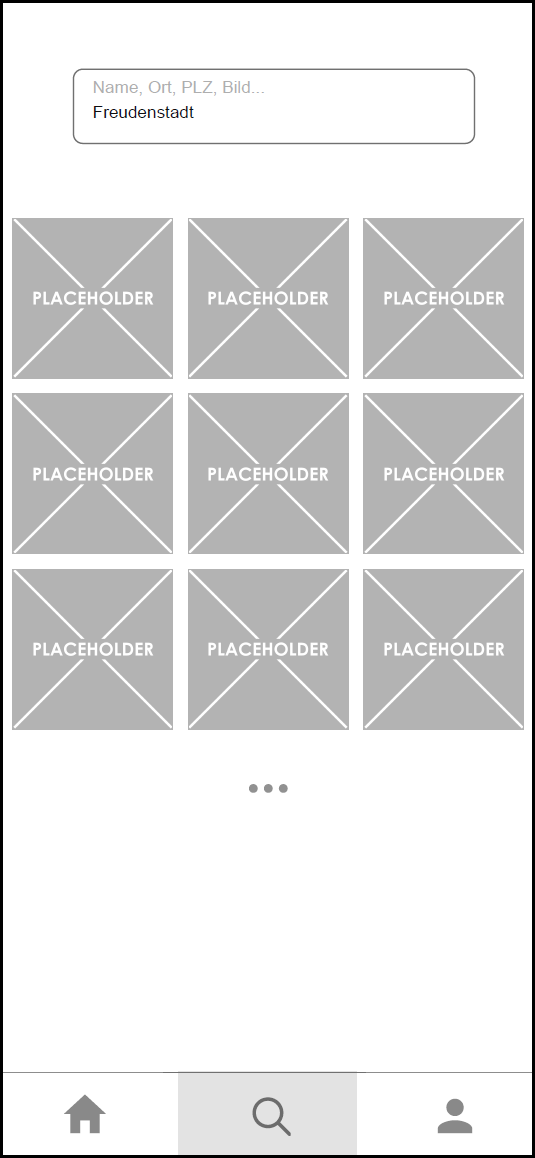
\includegraphics[width=.6\linewidth]{images/Feed_Overview_MockUp.png}
        \caption{Feed Overview}
        \label{fig:feed_overview}
    \end{minipage}%
    \begin{minipage}{.5\textwidth}
      \centering
      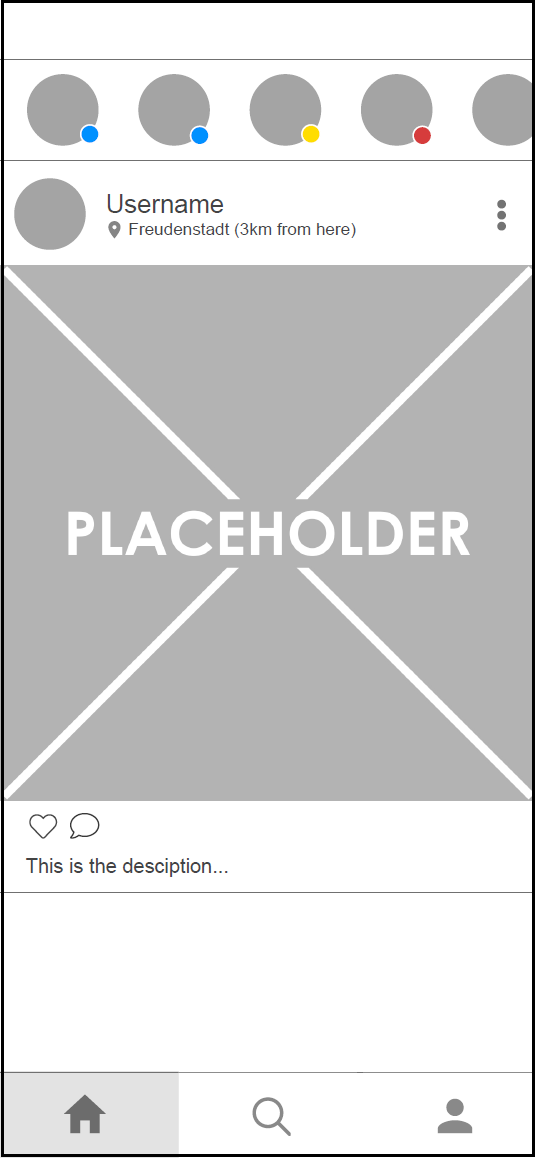
\includegraphics[width=.6\linewidth]{images/Feed_Detail_MockUp.png}
      \caption{Feed Detail}
      \label{fig:feed_detail}
    \end{minipage}
\end{figure}

Die folgenden zwei Abbildungen zeigen die Profilansicht mit Änderungsmöglichkeit.

\begin{figure}[H]
    \centering
    \begin{minipage}{.5\textwidth}
      \centering
      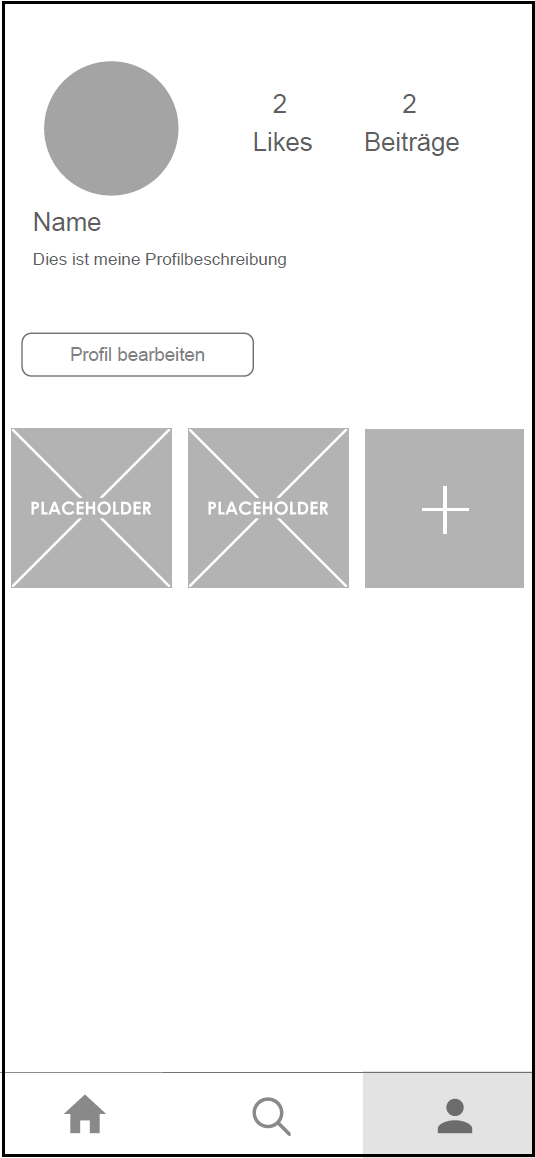
\includegraphics[width=.6\linewidth]{images/Profil_MockUp.png}
      \caption{Eigene Profil-Übersicht}
      \label{fig:own_profile}
    \end{minipage}%
    \begin{minipage}{.5\textwidth}
      \centering
      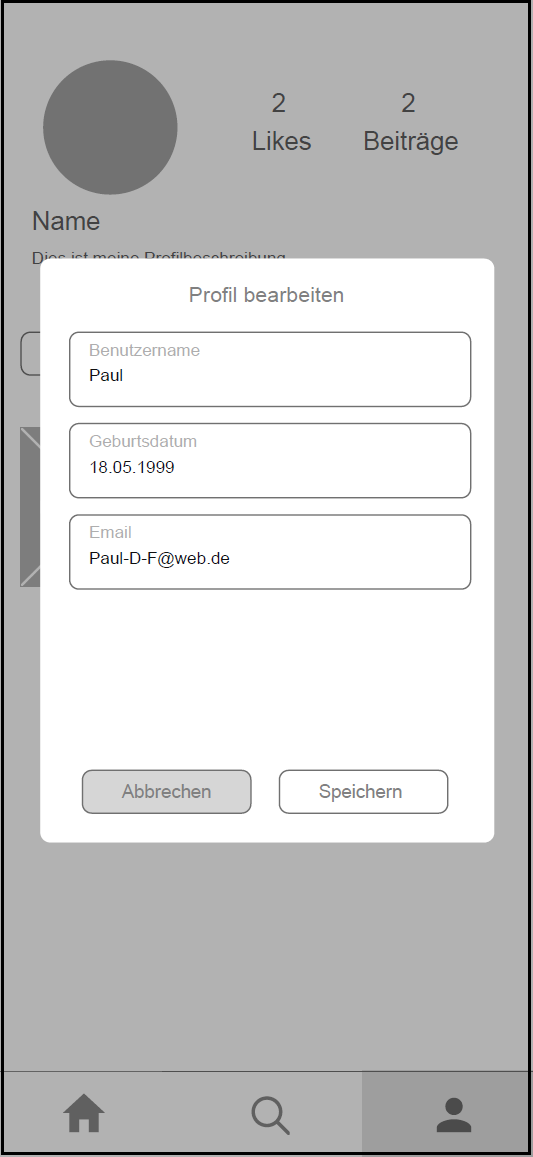
\includegraphics[width=.6\linewidth]{images/Edit_Profil_MockUp.png}
      \caption{Eigenes Profil bearbeiten}
      \label{fig:edit_profil}
    \end{minipage}
\end{figure}

Der Vorgang beim Hochladen eines neuen Feeds wird in \autoref{fig:popup_new_feed} und \autoref{fig:edit_new_feed} visualisiert. Der Benutzer hat die Möglichkeit das Foto entweder aus der eigenen Galerie auszuwählen oder mit der Kamera aufzunehmen. Noch während dem Hochladevorgang kann der Benutzer dem Feed eine Beschreibung und die GPS-Informationen für die Standortangabe hinzufügen.

\begin{figure}[H]
    \centering
    \begin{minipage}{.5\textwidth}
      \centering
      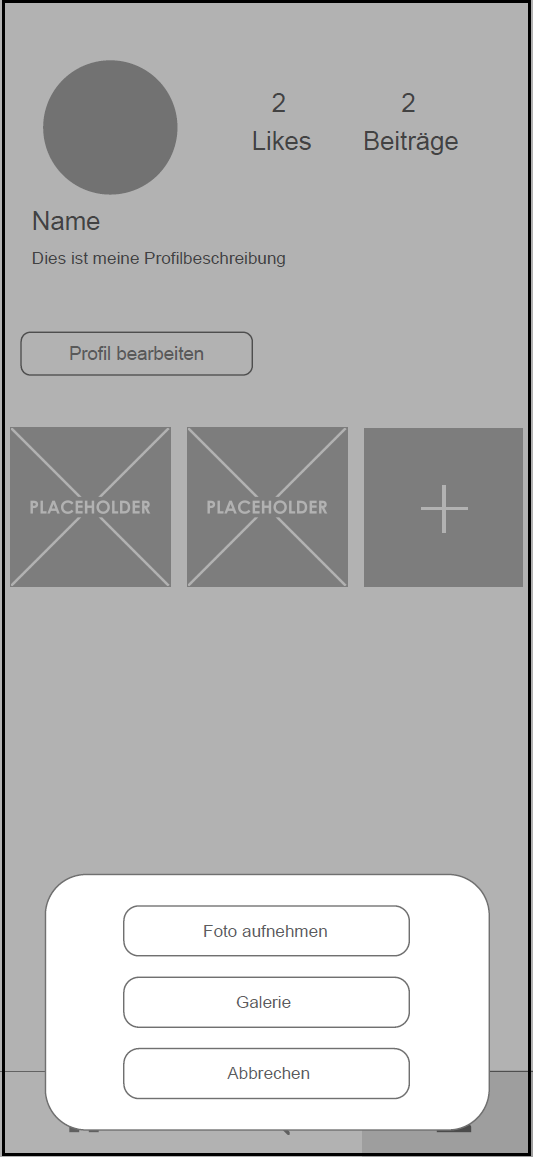
\includegraphics[width=.6\linewidth]{images/PopUp_Photo_MockUp.png}
      \caption{PopUp-Fenster für neuen Feed}
      \label{fig:popup_new_feed}
    \end{minipage}%
    \begin{minipage}{.5\textwidth}
      \centering
      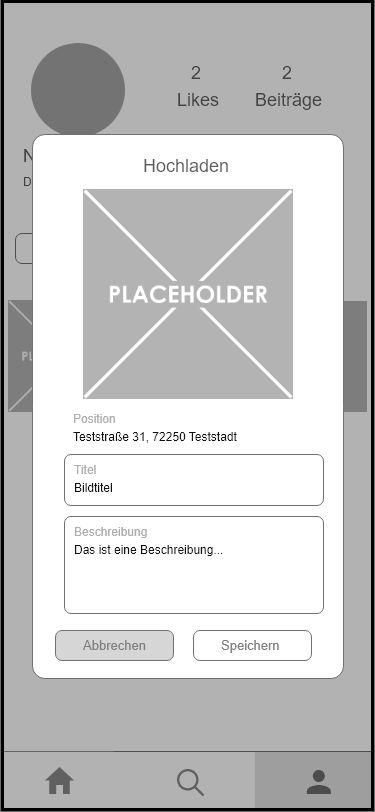
\includegraphics[width=.6\linewidth]{images/PopUp_Edit_New_Photo_MockUp.png}
      \caption{Neuen Feed bearbeiten}
      \label{fig:edit_new_feed}
    \end{minipage}
\end{figure}

\section{MVP-Kriterien\label{sec2.2:Unterpunkt-2}}

Folgende Kriterien müssen für eine erste, minimal funktionsfähige Iteration der mobilen Anwendung \glqq Geogram\grqq{}, während der Implementierung umgesetzt werden:

\begin{itemize}
    \item Login/Nutzerverwaltung
    \item Upload-Funktion für die Bilder mit Standortdaten
    \item Zugriff auf die Kamerafunktion des Mobilgerätes
    \item Zugriff auf die GPS-Daten (GPS-Modul des Mobilgerätes)
    \item Datenbank für Benutzerkonten, Standortdaten und Bildern
    \item Anzeigen der Beiträge
\end{itemize}

\section{Soll- und Kann-Kriterien\label{sec2.3:Unterpunkt-3}}

Neben den relevanten MVP-Kriterien wird die Konzeption noch mit Soll- und Kann-Kriterien ergänzt.

\textbf{Soll-Kriterien:}

\begin{itemize}
    \item Löschen von Bildern bzw. Beiträgen
    \item Hinzufügen von Bildbeschreibungen
    \item Ansicht des eigenen Kontos
    \item Einbindung von Google Maps für die Standortdaten
\end{itemize}

\textbf{Kann-Kriterien:}

\begin{itemize}
    \item Anmelden per Fingerabdruckssensor
    \item Anderen Benutzer "folgen" ("folgen"-Funktion)
    \item Benutzerdefinierte Filterfunktion für Beiträge
    \item Kommentare, Likes und Hastags für die Beiträge
    \item Dark-Mode abhängig von Systemeinstellungen
\end{itemize}